\documentclass[11pt]{article}
\usepackage{amsmath, amsthm, amssymb}
\DeclareMathOperator{\Tr}{Tr}
\usepackage{amsfonts}
\usepackage{amssymb,amscd}
\usepackage{array}
\usepackage{indentfirst}
\usepackage{graphicx}
\usepackage{color}
\usepackage{float}
\usepackage{url}
\usepackage{bm}
\usepackage[super]{natbib}
\usepackage{braket}
\usepackage{enumerate}
\usepackage{caption}
\usepackage[font={footnotesize}]{subcaption}
\usepackage[normalem]{ulem}
\usepackage[left=1.25in,top=1.5in,bottom=1in,right=1.25in, nohead]{geometry}
\usepackage[space]{grffile}
\usepackage{multirow}
\usepackage{longtable}
\usepackage{hyperref}
\usepackage{booktabs}

%\usepackage[T1]{fontenc}
%\usepackage{garamondx}
%\usepackage[garamondx,cmbraces]{newtxmath}

%\usepackage[urw-garamond]{mathdesign}
\usepackage[T1]{fontenc}

\def\RR{{\mathbb R}}
\def\CC{{\mathbb C}}
\def\NN{{\mathbb N}}
\def\ZZ{{\mathbb Z}}
\def\QQ{{\mathbb Q}}
\def\H{{\mathcal H}}


% Different font in captions
\newcommand{\captionfonts}{\normalsize}

\makeatletter  % Allow the use of @ in command names
\long\def\@makecaption#1#2{%
  \vskip\abovecaptionskip
  \sbox\@tempboxa{{\captionfonts #1: #2}}%
  \ifdim \wd\@tempboxa >\hsize
    {\captionfonts #1: #2\par}
  \else
    \hbox to\hsize{\hfil\box\@tempboxa\hfil}%
  \fi
  \vskip\belowcaptionskip}
\makeatother   % Cancel the effect of \makeatletter

\newtheorem{theorem}{Theorem}[section]
\newtheorem{corollary}[theorem]{Corollary}
\newtheorem{proposition}[theorem]{Proposition}
\newtheorem{lemma}[theorem]{Lemma}

\makeatletter
\newsavebox\myboxA
\newsavebox\myboxB
\newlength\mylenA

\newcommand{\exedout}{%
  \rule{0.8\textwidth}{0.5\textwidth}%
}
\newcommand*\xoverline[2][0.75]{%
    \sbox{\myboxA}{$\m@th#2$}%
    \setbox\myboxB\null% Phantom box
    \ht\myboxB=\ht\myboxA%
    \dp\myboxB=\dp\myboxA%
    \wd\myboxB=#1\wd\myboxA% Scale phantom
    \sbox\myboxB{$\m@th\overline{\copy\myboxB}$}%  Overlined phantom
    \setlength\mylenA{\the\wd\myboxA}%   calc width diff
    \addtolength\mylenA{-\the\wd\myboxB}%
    \ifdim\wd\myboxB<\wd\myboxA%
       \rlap{\hskip 0.5\mylenA\usebox\myboxB}{\usebox\myboxA}%
    \else
        \hskip -0.5\mylenA\rlap{\usebox\myboxA}{\hskip 0.5\mylenA\usebox\myboxB}%
    \fi}

\newcommand{\verbatimfont}[1]{\renewcommand{\verbatim@font}{\ttfamily#1}}

\makeatother

\setlength{\intextsep}{10pt plus 2pt minus 2pt}
\title{Citrine Test Problem: Alloy Stabilities}
\author{Aidan Klobuchar}
\date{}
\begin{document}
\maketitle
\section{Introduction/Project Gameplan}
\noindent
Given the promising and large search space alloys allow scientists to explore for the development of new catalysts or other materials (semiconductors, etc.), being able to accurately and cheaply predict the stability of a large variety of alloy types and compositions would be a great screening tool. Machine learning, allowing us to skip the need to perform costly electronic structure calculations while still maintaining a high level of accuracy, is a promising avenue for creating such a predictor. Building such a prediction framework would be best handled in an iterative manner, making sure that the stabilities of simpler alloys can be predicted accurately before moving on to more complex cases. With that said, this exercise functions as the first step to such a predictor, by attempting to predict whether not various binary alloys are stable or not. This ignores the complications of phase diagrams, beyond binary alloys, novel compositions or geometries, and any detailed energetics. Still, if this task cannot be accomplished, than the more complicated ones will stay out of reach. 
\\
\\*
The first task to solving this problem is to create and investigate a gameplan for tackling the problem. to begin to accomplish this, we should first perform some exploratory data analysis. The first step is to impose a slight bit of structure on our dataset. Our dataset consists of pairs of a variety of atomic and chemical properties for two candidate elements, labelled `A' and `B'. However, the order of `A' and `B' is totally arbitrary. Thus, going forward, I will use a reordered version of the dataset, where the atomic volume of A is always greater than the volume of B. Now, given that our target is essentially the Boolean stabiliites for 9 alloy configurations (given that the 0 \% and 100 \% cases are always stable) per pair of metals, it would be useful to determine the correlations between these alloy configurations, to determine the feasibility of solving 9 independent, smaller problems, instead of solving a single larger problem. This correlation matrix is shown as \eqref{eq:stab_corr}, where all correlations are below 33 \%, with most being less than 15 \%, demonstrating the feasibility of such an approach. Given that there \emph{are} still correlations between the stabilities of different compositions, figuring out how to incorporate these correlations into the final results is another avenue to keep in mind. 
\begin{align}
\label{eq:stab_corr}
SC &= \begin{bmatrix}
1.00 & 0.14 & 0.14 & -0.02 & 0.04 & 0.00 & -0.04 & -0.01 & -0.02 \\
0.14 & 1.00 & 0.18 & 0.10 & 0.28 & 0.09 & 0.17 & -0.04 & -0.01 \\
0.14 & 0.18 & 1.00 & 0.12 & 0.32 & 0.15 & 0.09 & 0.11 & 0.03 \\
-0.02 & 0.10 & 0.12 & 1.00 & 0.21 & 0.16 & 0.16 & 0.00 & -0.02 \\
0.04 & 0.28 & 0.32 & 0.21 & 1.00 & 0.21 & 0.20 & 0.07 & 0.05 \\
0.00 & 0.09 & 0.15 & 0.16 & 0.21 & 1.00 & 0.13 & 0.08 & -0.02 \\
-0.04 & 0.17 & 0.09 & 0.16 & 0.20 & 0.13 & 1.00 & 0.15 & 0.06 \\
-0.01 & -0.04 & 0.11 & 0.00 & 0.07 & 0.08 & 0.15 & 1.00 & 0.14 \\
-0.02 & -0.01 & 0.03 & -0.02 & 0.05 & -0.02 & 0.06 & 0.14 & 1.00
\end{bmatrix}
\end{align}

\noindent The next task is to look for potentially simple but informative some problems. For example, if a metal pair has no stable alloy compositions, it is reasonable to assume that it may have some obviously unique or mismatched descriptors, leading this to be a promising early avenue of investigation. Checking the prevalence of the number of stable alloys per metal pair, we end up with Fig.~\ref{alloy_comp_bar}. Here we see that over \emph{half} of the metal pairs (1344/2572) contain no stable alloys. Thus, being able to predict whether or not \emph{any} stable alloys will form is a great place to start; not only is it likely a simpler subproblem, but solving it will aid in solving the more finegrained fractional alloy stabilities, as a lot of unstable alloys (zeros in target vectors) will be removed, allowing for more balanced classes, leaving us with one less thing to deal with (there are ways to deal with heavily unbalanced classes, but avoiding additional complications seems ideal). 

\begin{figure}[H]
\centering
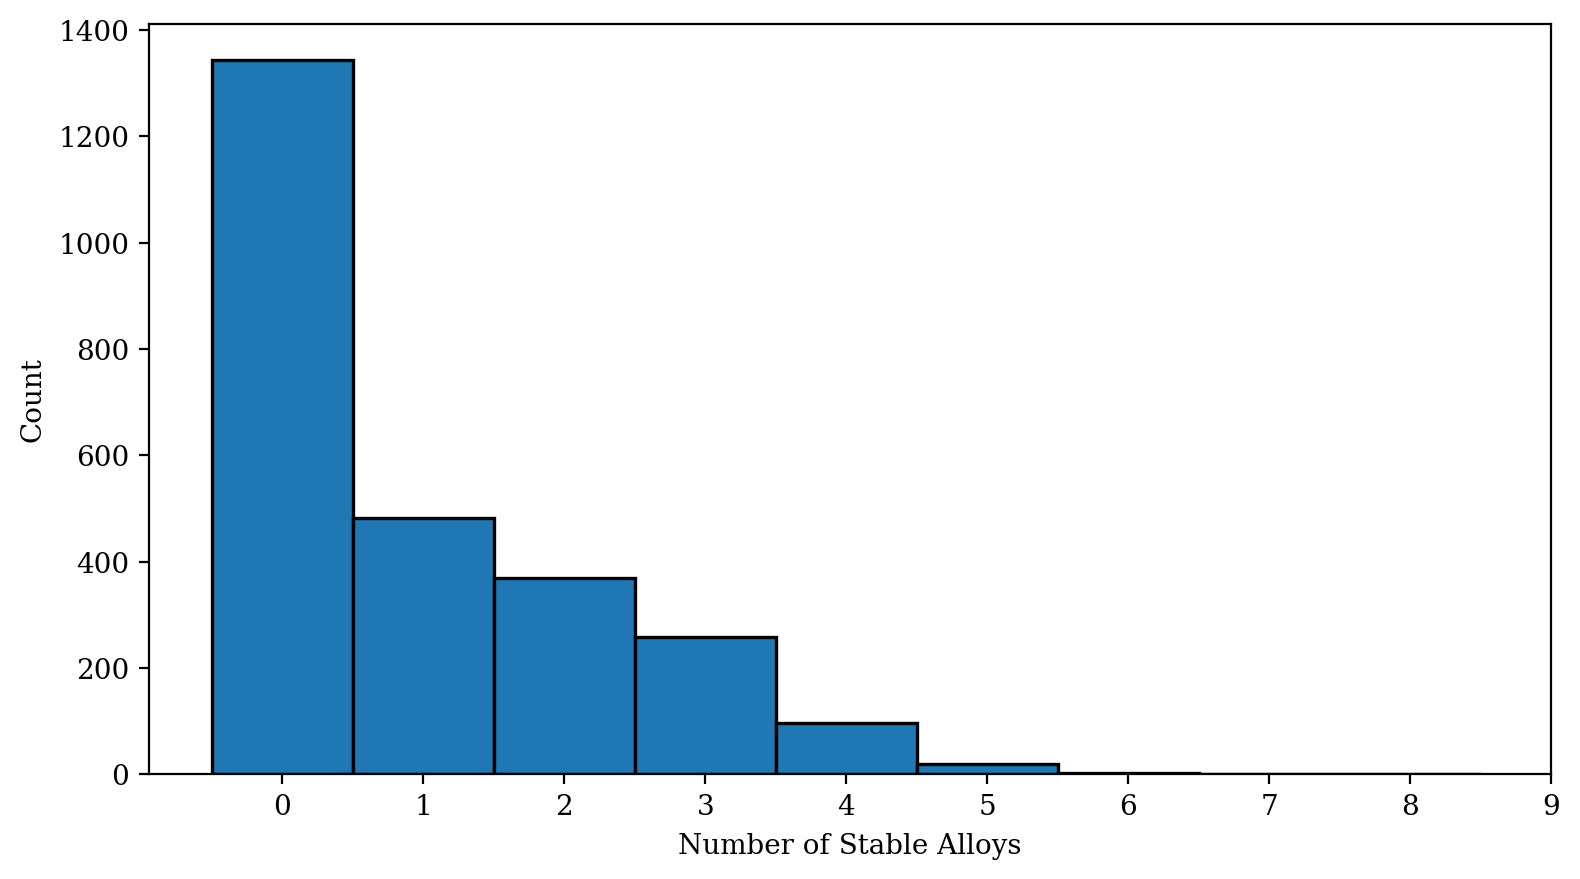
\includegraphics[width=0.7\textwidth]{stable_suballoys_hist.png}
\caption{Number of Stable Alloy Compositions per Metal Pair}
\label{alloy_comp_bar}
\end{figure}

\noindent Assuming the simpler Boolean alloy problem is solved, we will be left with some number of alloys that should produce one or more stable alloys. Thus the next task is to solve the 9 different alloy composition classification problems. However, trying to investigate and tune nine separate but likely highly similar classification problems is unwieldy and inefficient. Thus we want to look at a couple of informative and populated alloy classes to investigate the most closely. Looking at a plot of the commonality of the different alloy compositions (Fig.~\ref{alloy_comp_hist}), we see that 30 \% and 50 \% of A cases are the most populated, so those are the ones I will investigate more closely. After a few candidate classifiers are identified for these two cases, they will be tested on the full set of 9 compositions. These predictions can then be modified based on the correlations seen in \eqref{eq:stab_corr}. Finally, all pieces of the problem can be tackled in one go, to get a final error estimate. This give us the following roadmap:
\begin{itemize}
\item Solve Boolean alloy stability problem.
\begin{itemize}
\item Determine appropriate descriptors.
\item Test various classification models.
\item Tune hyperparameters.
\end{itemize}
\item Investigate 30 \% and 50 \% A cases.
\begin{itemize}
\item Determines/create descriptors.
\item Test and tune classifiers.
\end{itemize}
\item Test on full 9 alloy problem space.
\item Modify predictions based on stability vector correlations. 
\item Test entire problem flow.
\end{itemize} 

\begin{figure}[H]
\centering
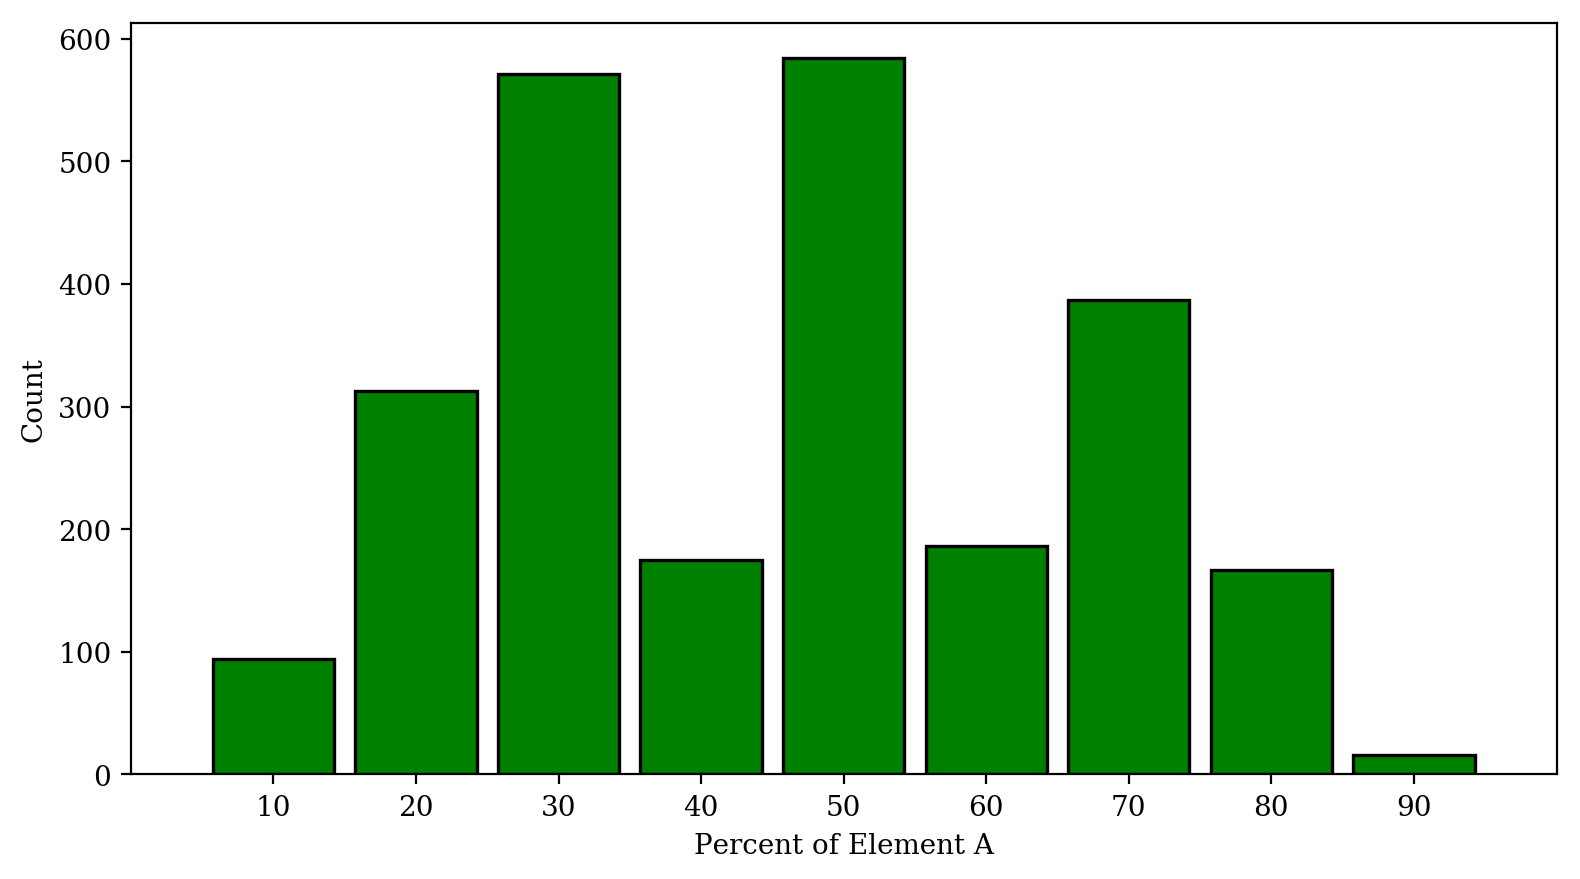
\includegraphics[width=0.7\textwidth]{alloy_composition_bar_chart.png}
\caption{Number of Stable Alloys per Composition Percentage}
\label{alloy_comp_hist}
\end{figure}

\section{Boolean Compound Problem}
\subsection{Descriptor Determination and Development}
\noindent The first, and arguably most difficult, step in tackling our classification problems is to take our dataset containing with 96 different properties and turning them into a smaller and representative set of descriptors that we can use for fitting while hopefully avoiding overfitting or noise from an overly large descriptor set. Given that all of the properties we care about come in pairs, it makes sense to create new descriptors based on performing the various binary operations (addition, subtraction, multiplication, division) on our descriptor pairs. Furthermore, it also makes sense to take the absolute value of the differencr as a sort of $l_1$ distance metric. Doing so creates $48*5 = 240$ additional descriptors, leading to a total of 336 candidates to whittle down, which were then standardized (mean and standard deviation 1 for each descriptor). I decided to use two metrics in determining which descriptors to use or discard. The first was the correlation coefficient of the descriptor with the target Boolean vector (0 if the metal pair forms no stable alloys, 1 otherwise), whose absolute value can range from 0 to 1. The exact distribution of these values can be seen in Fig~\ref{bool_corr_hist}. 

\begin{figure}[H]
\centering
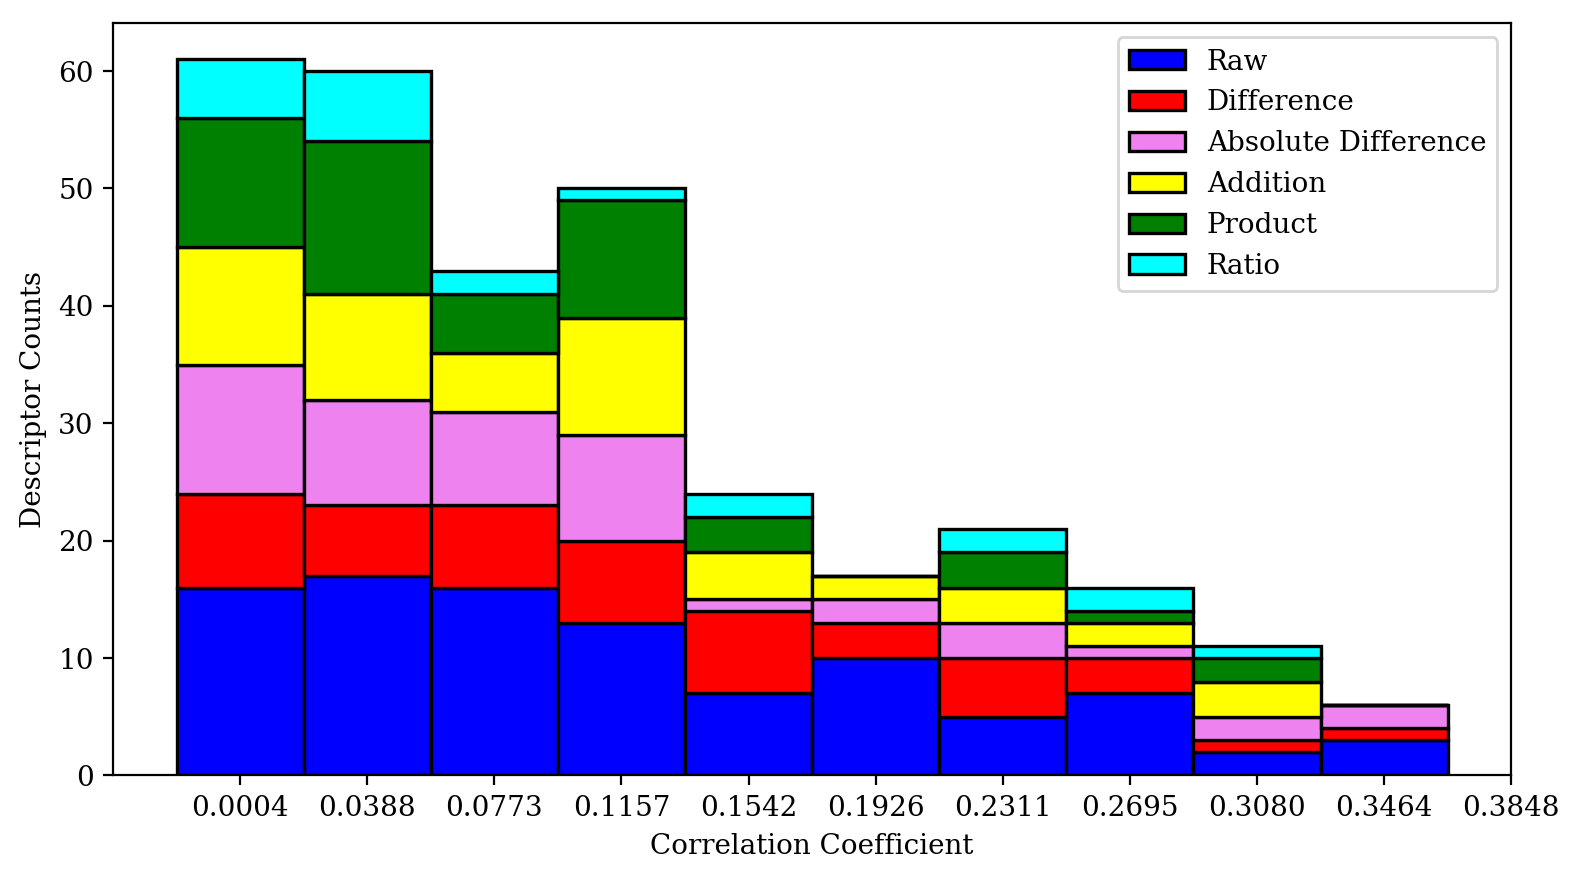
\includegraphics[width=0.7\textwidth]{descriptor_correlations_hist.png}
\caption{Absolute Correlations Between Descriptors and Boolean Alloy Stability Vector}
\label{bool_corr_hist}
\end{figure}

\noindent The second metric would be the correlation of a descriptor with other descriptors, as we do not wan sets of highly correlated descriptors. While I did investigate this manually quite a bit, I used this to create an automatic method, where only the vectors that have a decent correlation with the target is considered. Then, of those, between every highly correlated pair of descriptors, the one that is most correlated with the other descriptors is removed. With the parameters I used, this led to 59 descriptors being used; still somewhat unwieldy, but at least somewhat manageable. With more time, I might investigate tightening up some of the requirements to produce a smaller descriptor set. I then further reduced this set using principal component analysis, generally keeping enough descriptors to keep 90 \% of the explained variance. 

\subsection{Classifier Tests}

\noindent With a set of promising descriptors in hand, the next step is to test a variety of classifiers and hyperparameters. In order to avoid too much bias from overfitting to the training set, I used five fold cross validation to approximate the out of training set error, fitting a variety of classifiers on five 80 \% splits of the data and then testing on the held out 20 \% of the dataset. In order to determine model performance, I relied on using the F1 score, which is the harmonic mean of the model's precision and recall, of the weighted average of the two possible classes. I also looked at the RMSE of the probabilities the model determined as compared to the certain ground truth. I tested logistic regression, SVM classifiers, Gaussian Process classifiers (the latter two both using a radial basis function kernel), decision tree classifiers, and random forest classifiers. These were tested using a variety of hyperparameters with and without the use of PCA dimensionality reduction. Cutting a long and data filled story short, I found that SVM and random forest classifiers performed best, with RMSE probability errors of around 0.3 and F1 scores around 0.87. The best SVM classifiers had values of C around 1.0 with a gamma value around 0.5, while the best random forest classifiers had max depth of around 15, used the 'gini' splitting criteria, and used 25 decision tree estimators.
\\
\\*
(NOTE: There was a bug in the cross validation code from an older project, so many of the saved f1 values are wrong; they are basically NOT cross validated, though the accuracy RMSE values should be correct)

\section{Alloy Composition Stability Problem}
\subsection{Descriptor Development and Selection}
\noindent While the general framework/ideas for solving this problem, given the results of the previous Boolean problem, are similar to the methods above, there are some differences in the choice of descriptors. For one, we are now dealing with a variety of different fractional configurations. And now that we are concerned with how the different atoms can bind, we need to consider electrons and electron counts. Now there isn't a particularly clean way of doing, but I settled on creating lists of feasible valence electron and hole counts for each element. The reason for multiple counts can be seen with something that has the configuration 4s$^1$3d$^4$, which could feasibly want to accept 1 (to fill the s or half fill the d shell), 2, 6 or 7 (filling both shells) electrons. Thus, with these lists constructed for every element, I looked for the smallest mismatch between the available and needed electrons, modulated by the fraction of elements A and B in the composition. I also looked solely at the configurations I thought were best and at the valence similarities between different components, neither of which were as significant a descriptor as the more grab bag approach. 
\\
\\*
On top of the electron `fit' discussed above, I looked both at fractionally weighted and raw descriptors for the full descriptor space (until VERY recently, I was using just a subset of the space, hence Fig.~\ref{alloy_corr_hist}). I then attached the electron descriptor(s) to these and pruned the descriptors as above for each alloy composition problem, keeping those descriptors that were deemed significant for at least 6 of the 9 problems. Doing this brought us from 674 descriptors down to 49. The full spread of the correlation values for the old case of using the best subset of alloy descriptors, with 26 candidate descriptors lumped together for each of the 9 alloy problems is shown in Fig.~\ref{alloy_corr_hist}.

\begin{figure}[H]
\centering
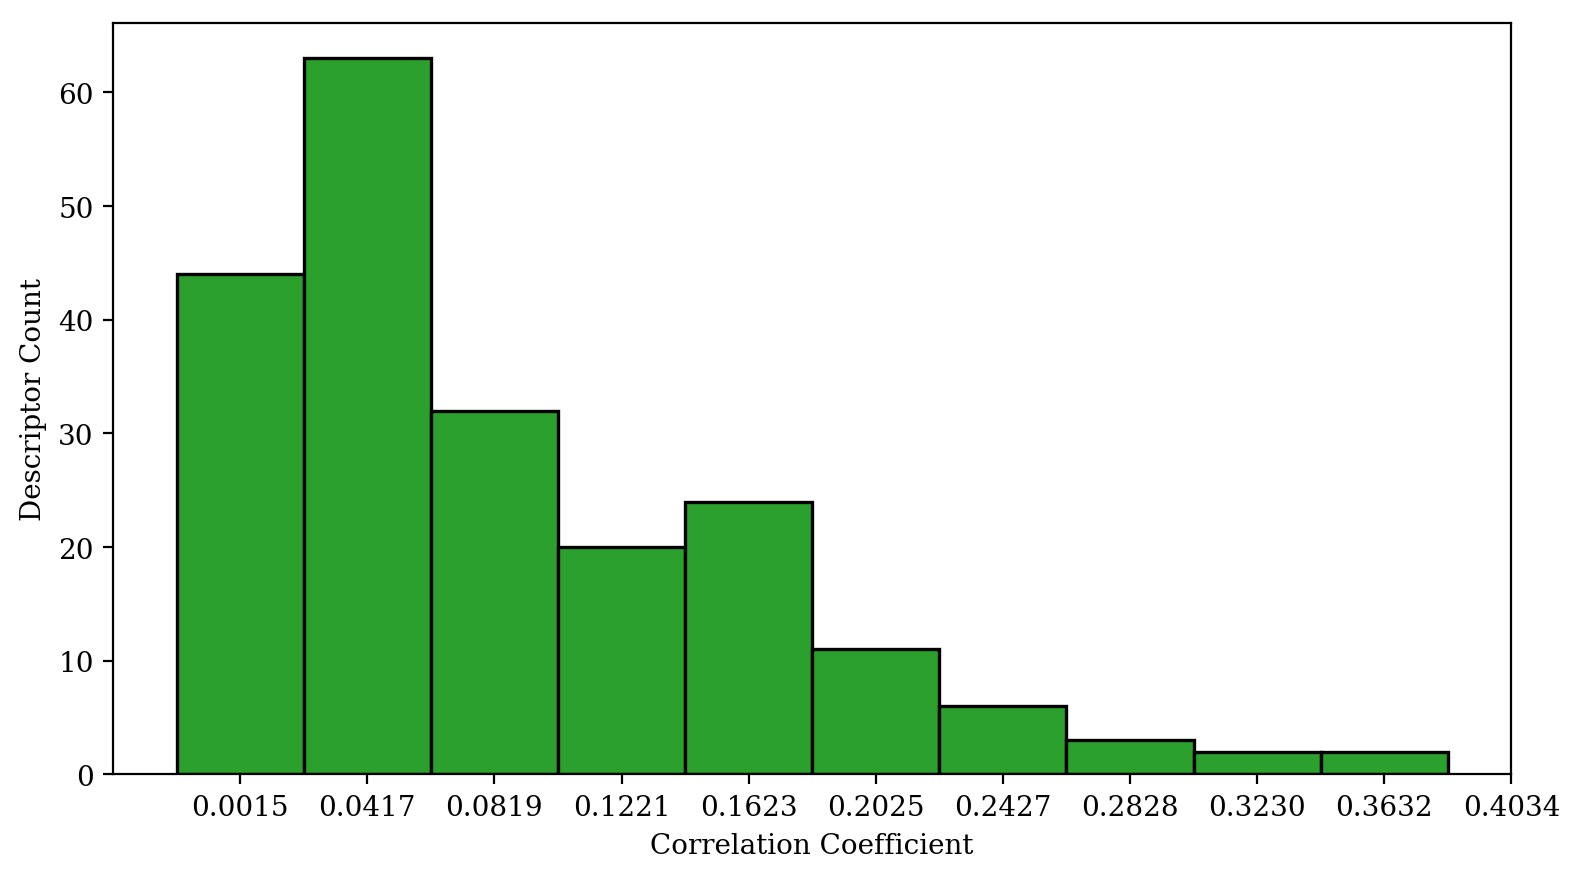
\includegraphics[width=0.7\textwidth]{alloy_comp_descriptor_hist.png}
\caption{Absolute Correlations Between Each Set of Alloy Descriptors and the Matching Alloy Composition Stability Vector}
\label{alloy_corr_hist}
\end{figure}

\subsection{Alloy Classification}
\noindent With a small set of meaningful descriptors in hand and the methodology for testing various classifiers already developed, this subproblem is pretty straightforward, with the only real issue being the accumulation and analysis of the produced data. As discussed earlier, the `larger' 30 \% and 50 \% cases were investigated first to narrow down the choice of classifiers, with SVM classifiers, decision tree classifiers, and random forest classifiers again taking the lead spot, with the decision tree classifiers being thrown away due to my fear of their penchant for overfitting the data. Afterwards, a smaller set of classifiers were run for all 9 stability compositions, running with and without additional PCA dimensionality reduction. Doing so, we find the best classifiers to have probability RMSEs between 0.1 and 0.43 and f1-scores between 0.71 and 0.98, depending on which of the nine classification problems we look at (the larger, 30 \% and 50 \% do poorly, while cases such as the 10 \% case do well). These results (due in part to the aforementioned cross validation coding error) do raise into question the nature of the descriptors used, though the results aren't too bad for a first pass. 

\section{Finalization and Estimated Prediction Errors}
\subsection{Probability Modification}
\noindent While the stability of each alloy composition is determined independently from the rest, we know that this is an approximation, given the correlation values present in \eqref{eq:stab_corr}. Thus it would nice, at least in a theoretical sense, to modify the predictions produced by the independent classification problems using the correlations between the different alloy compositions. To do this , I used the probabilities of being stable, as computed by the classifiers we are testing, and modified them according to \eqref{stab_corr_mod}, where $P_{stab}$ is new 9 element stability probability vector, $p_{stab}$ is the original vector (where the probabilities have been scaled to lie within the range [-1,1] for each), and $SC$ is the correlation matrix from \eqref{eq:stab_corr}. The idea is to add or subtract from the probability based both on the strength of both the stability vector correlation and the certainty of alloy composition prediction. This modification is scaled by the $ \left(1-\textrm{sign}(SC_{ij})*p^i_{stab}*\textrm{sign}(p^j_{stab})\right)$ term, so that prediction/correlation combination that pull the prediction to 0 (so 50/50) have a larger influence than those that pull it to the -1/1 extremes. 
\begin{align}
\label{stab_corr_mod}
P^i_{stab} =(1/8) * \sum_{i\neq j}^{9} \left(1-\textrm{sign}(SC_{ij})*p^i_{stab}*\textrm{sign}(p^j_{stab})\right)*0.5*SC_{ij}*p^j_{stab}
\end{align}

\subsection{Final Tests and Error Estimation}
\noindent The penultimate step in the solution of this problem is obtain reasonable estimates for the performance of the model on outside data and to pick a final set of classifiers to use. As a first step in this process, and as a sanity check, I ran the entire process on the training set to make sure that the various error metrics for the training data were reasonable. Next, I took the best couple of classifier sets and estimated the error on outside data using .632 bootstrapping. Here, samples are drawn with replacement from the training data to used to create classifier fits, while the data that is randomly left out is used as test data to estimate the outside error. Because this bootstrapping process uses only around 63 \% of the data, it tends to be pessimistic, and is thus modified by adding in some of the overly optimistic full training error. In equation form, this gives,
\begin{align}
\label{BS}
\widehat{\textrm{Err}}^{(BS)} &= \frac{1}{N_B}\sum_{N_B}\frac{1}{N_i}\sum_{x_i \notin \tilde{D}}L(y_i, f^{\tilde{D}}(x_i))\\
\overline{\textrm{err}}& =\frac{1}{N_D} \sum_{D} L(y_i, f(x_i))\\
\widehat{\textrm{Err}}^{(.632)} &= 0.632 \cdot \widehat{\textrm{Err}}^{(BS)} + 0.368 \cdot \overline{\textrm{err}},
\end{align}
where $N_B$ is the number of bootstrap samples taken (I used 150), $D$ is the full dataset, $y$ is the target vector, and $L()$ is the loss function for whatever error metric is being considered. Running this, we get the following probability RMSE values, precisions, recalls, f1 scores, and total accuracies:

\begin{table}[h!]
\caption{Raw Bootstrap Test Error Metrics}
\label{bs_res}
\vspace{3mm}
\centering
\begin{tabular}{lccc}
\toprule
\multicolumn{1}{l}{Percent of Element A}  & \multicolumn{1}{c}{Precision} & \multicolumn{1}{c}{Recall} & \multicolumn{1}{c}{F1-Score} \\
\midrule
10 \% & 0.958 & 0.966 & 0.960 \\
20 \% & 0.854 & 0.874 & 0.861 \\
30 \% & 0.832 & 0.830 & 0.831 \\
40 \% & 0.927 & 0.939 & 0.929 \\
50 \% & 0.819 & 0.820 & 0.820 \\
60 \% & 0.910 & 0.929 & 0.914 \\
70 \% & 0.853 & 0.864 & 0.857 \\
80 \% & 0.906 & 0.928 & 0.914 \\
90 \% & 0.989 & 0.993 & 0.991 \\
\bottomrule
\end{tabular}
\end{table}

\begin{table}[h!]
\caption{0.632 Bootstrap Test Error Metrics}
\label{632_res}
\vspace{3mm}
\centering
\begin{tabular}{lccc}
\toprule
\multicolumn{1}{l}{Percent of Element A}  & \multicolumn{1}{c}{Precision} & \multicolumn{1}{c}{Recall} & \multicolumn{1}{c}{F1-Score} \\
\midrule
10 \% & 0.973 & 0.978 & 0.974 \\
20 \% & 0.907 & 0.919 & 0.911 \\
30 \% & 0.893 & 0.892 & 0.893 \\
40 \% & 0.953 & 0.960 & 0.954 \\
50 \% & 0.886 & 0.886 & 0.886 \\
60 \% & 0.942 & 0.954 & 0.945 \\
70 \% & 0.906 & 0.913 & 0.909 \\
80 \% & 0.940 & 0.953 & 0.944 \\
90 \% & 0.993 & 0.996 & 0.994 \\
\bottomrule
\end{tabular}
\end{table}

\begin{table}[h!]
\caption{Averaged 0.632 Bootstrap Test Error Metrics}
\label{avg_632_res}
\vspace{3mm}
\centering
\begin{tabular}{lc}
\toprule
\multicolumn{1}{l}{Metric}  & \multicolumn{1}{c}{Average Value}  \\
\midrule
Precision & 0.932 \\
Recall & 0.939 \\
F1-Score & 0.934 \\
Percent Wrong & 6.10 \% \\
\bottomrule
\end{tabular}
\end{table}


\section{Test Set Results and Concerns}
\noindent 
Using the final classifier set, random forest classifiers with a maximum depth of 15 and 25 estimators for both the Boolean and the alloy problem, stability vector prediction were created for the provided holdout test set. where only around 300 element pairs were predicted to have stable alloys, a somewhat lower percentage than for the training set. Whether or not this is actually a concern, as the test set was never said to have similar behavior to the training set, it is still worth noting. This of course raises an ever present concern in machine learning; if the test set contain elements or element pairs that behave in fundamentally different way than anything in the training set (or even if said behavior was just very underrepresented), how can we possibly guarantee an accurate handling of those data points? For example, dealing elements such as Helium (that have, of course, no melting point...). Still, while I cannot be fully confident of how my model handles the more extreme or exotic element combinations, due to having weird sets of properties that may not have shown up in the test set, I do feel pretty good about the predicted results. Unfortunately, since I do not have any real alloy stability data on hand or in my head, I have no way to really sanity check the results. In addition, when using models more complex than simple linear models, the risk of overfitting, especially when using larger descriptor spaces, is always a worry, even after using cross validation and bootstrapping techniques to try and prevent this. 

\section{File List:}
\begin{itemize}
\item citrine\_code.py: All of the python methods used to produce this work.
\item fit\_test\_data.csv: The test data with the current set of stability vector predictions.
\item final\_class\_dict.pckl: A dictionary containing all of the objects needed to run the stability vector predictor on new data.
\item new\_bs\_res.pckl: File containing the results/metrics from the most recent bootstrap run.
\item alloy\_script\_test2  (and 3).pckl: Files containing the most recent results for running a few classifiers for all 9 alloy problems.
\item Four png files: Graphs used/described in this writeup.
\item test\_data\_1.csv Outdated predictions for the test sets stability vectors (using the too small alloy descriptor matrix).
\item compound\_yes\_no\_results.pckl: File containing somewhat outdated (I think?) results from the Boolean classification problem.
\item alloy\_x\_tree.png/.dot: Images or files containing image data for some of the earlier trees fitted to the alloy 30 \% and 50 \% problems. Are too big to be very intuitively useful.
\item alloy\_class\_results.pckl: Old results from running the 30 and 50 \% alloy problems.
\item Anything with `mat' or 'matrix' in the title: Old files saving test descriptor matrices before I just automated the process.
\item correlations\_?.pckl: Files containing descriptor/Boolean target correlations.
\item compound\_boolean.pckl: Target vector for the Boolean classifier problem.
\item stability\_vectors.pckl: Target for the alloy classifier problems.
\item ordered\_training\_data.csv: Training data with element A always having the larger volume.
\end{itemize}

\end{document}